%                                                                 aa.dem
% AA vers. 9.1, LaTeX class for Astronomy & Astrophysics
% demonstration file
%                                                       (c) EDP Sciences
%-----------------------------------------------------------------------
%
% \documentclass[referee]{aa} % for a referee version
%\documentclass[onecolumn]{aa} % for a paper on 1 column  
%\documentclass[longauth]{aa} % for the long lists of affiliations 
% \documentclass[letter]{aa} % for the letters 
%\documentclass[bibyear]{aa} % if the references are not structured 
%                              according to the author-year natbib style

%
\documentclass{aa}  

%
\usepackage{amsmath}
\usepackage{graphicx, comment}
\usepackage{commath}
\usepackage{txfonts}
\usepackage{subfig}
\usepackage{upgreek}
\usepackage{threeparttable} 
\usepackage{booktabs}
\usepackage{siunitx}
\usepackage{natbib}
\usepackage{float}
\usepackage{enumitem}

% \usepackage[backend=biber, style=authoryear, natbib=true]{biblatex}
% 超链接配置：确保链接颜色可见，去除边框
\usepackage[colorlinks=true, linkcolor=blue, urlcolor=blue, citecolor=blue]{hyperref}
\usepackage{orcidlink}

\newcommand{\C}{3C\,84}
\newcommand{\rotang}{-4.5^\circ}
\newcommand{\protang}{4.5^\circ}
\newcommand{\beam}{(0.17\times0.40)\,\textrm{mas}}

\newcommand{\Mj}{5.0\pm1.7}
\newcommand{\Mjrel}{6.7\pm2.0}
\newcommand{\Mx}{9.8\pm3.2}
\newcommand{\enthalpy}{0.26\pm0.20}
\newcommand{\ajj}{0.14\pm0.06}
\newcommand{\ax}{0.07\pm0.02}
\newcommand{\bw}{0.27\pm0.04}

\newcommand{\rj}{0.36\pm0.09\,\textrm{pc}}
\newcommand{\phij}{4.5^\circ\pm1.2^\circ}
\newcommand{\thetaj}{35^\circ\pm5^\circ}
\newcommand{\gj}{1.35\pm0.14}


\newcommand{\tp}{30\pm10\,\textrm{years}}
\newcommand{\chiamp}{\sim1}
\newcommand{\chialt}{\sim2}




\begin{document} 

\renewcommand{\arraystretch}{1.5}
   
    \title{
    % 1.4GHz下对低红移射电星系的统计：用多种视角观察射电星系的特性
    Topic: \\Paper Name 
    }

    \author{
        P.-G. Zheng\inst{1,2}
    \and R.-Y. Ma\inst{1,2}\thanks{Corresponding author: \email{ryma@xmu.edu.cn}}
    \and Z.-H. Zhu\inst{3,2}\thanks{Corresponding author: \email{}}
    \and X. Cao\inst{1,2}
    \and Y. Xie\inst{4}\thanks{Corresponding author: \email{xieyi@jmu.edu.cn}}
    \and X.-L. Wang\inst{1,2}
    }
    
    \institute{
    Department of Astronomy and Institute of Theoretical Physics and Astrophysics, Xiamen University, Xiamen, Fujian 361005, China
    \and
    SHAO--XMU Joint Center for Astrophysics, Xiamen, Fujian 361005, China
    \and
    Shanghai Astronomical Observatory, Chinese Academy of Sciences, 80 Nandan Road, Shanghai 200030, China
    \and
    School of Science, Jimei University, Xiamen 361021, Fujian Province, China
    }




   \date{Received -; accepted -}


 \abstract
   {
   Radio Galaxies (RGs) are critical active galaxies driving cosmic structure evolution, with jet lobes as key components shaped by interactions with the circumgalactic medium. This study focuses on extracting morphological parameters of Fanaroff-Riley (FR)\textemdash classified RGs (FRI and FRII) from 1.4 GHz radio images via elliptical structure fitting, aiming to systematically characterize their morphological properties. To achieve this objective, a semi-automated workflow is developed to localize RG cores and lobes. Statistical analyses of the derived parameters reveal that both FRIs and FRIIs exhibit a peak axial ratio of approximately 0.25. Notably, FRII RGs possess larger intrinsic physical scales, with the scale distribution peaking at ~200 kpc, whereas the peak scale of FRIs is ~50 kpc. For FRI RGs, the number of knot structures shows a steady decreasing trend within specific brightness intervals. For FRII RGs, a distinct subclass structure emerges in the classification parameter space when $(r_s < 0.4)$, which is attributed to the regulatory effect of hot spot outflows. Furthermore, the stacked curve of the central line brightness of FRII RGs is consistent with the predicted dynamical evolution model of jet-cocoon expansion. These results validate the effectiveness of elliptical structure fitting in describing RG morphologies and provide critical insights into the intrinsic differences between FRI and FRII types. This work establishes a solid foundation for refining RG classification systems and advancing our understanding of active galactic nucleus (AGN) feedback processes in cosmic evolution. 
   }
 
  

   \keywords{
            Active galactic nuclei; Radio galaxy; Radio astronomy
               }

   \maketitle


\section{Result}\label{sec:Result}    
\subsection{The Statistical Characteristics of Geometric Parameters}\label{sec:Section4_1}

In order to compare with previous results and validate our results, we first show the $r_s$ function in \autoref{fig:Figure12} for FRIIs. 
It can be seen that our results agree with \citet{lin_populations_2010}, both showing two significant peaks around 0.15 and 0.60. 
Although there is a gap between 0.2 and 0.4 and some minor peaks around 0.5 and 0.8 in our results, the difference are acceptable. On the one hand, we excluded some sources as mentioned in previous section while their sources are more than those given by FIRST. On the other hand, the way we determine the value of $r_s$ for all the sources is the same, while \citet{lin_populations_2010} use different ways for different types of sources.
\textbf{Here the sources with $r_s<0.3$ should be not identified with $r_s$ \citep{}. These sources shows close radio knots and weak emission extending long distances.}
Notably, the $r_s$ distribution of FRIs presented in this work is consistent with that reported by \citet{lin_populations_2010}.

% 具体$r_s<0.3$的讨论和下面这一段一起讨论
%In \autoref{sec:Section3_6}, we reference the methodology for FR-type classification proposed by \cite{lin_populations_2010}, wherein FRIIs exhibit distinct and independent features in the region where $r_s < 0.3$. Building upon this methodology, we identify distinct subclass structures in this region. For $r_s < 0.3$, the distance between the two hot spots is considerably smaller relative to the overall size of the radio structure. However, targeted manual sampling of the dataset in this study reveals that this feature primarily stems from relatively prominent "outflow" structures: clumps centered on the hot spots extend outward in various directions. If such extension does not align with the optical counterpart (or central clump), the algorithm will expand the size of the ellipse to meet the specified coverage rate during fitting, ultimately resulting in a remarkably small hot spot distance relative to the major axis of the ellipse. 


%However, is an excessively stringent coverage rate the primary factor affecting the fitting of elliptical Gaussian components for hot spots? In the procedures illustrated in \autoref{fig:Section3_6}, we gradually reduced the coverage rate of the elliptical Gaussian components (with the coverage rate set to 95\%, 90\%, 80\%, 70\%, 60\%, and 50\% respectively), and observed that the positions of the peaks and the overall distribution remained stable. With the reduction of coverage constraints, the faint outflows on both sides of the lobes are the first to be excluded from the ellipses; but, it is evident that they do not significantly affect the stability of the subclass structures.


\begin{figure}[!htbp]
    \centering
    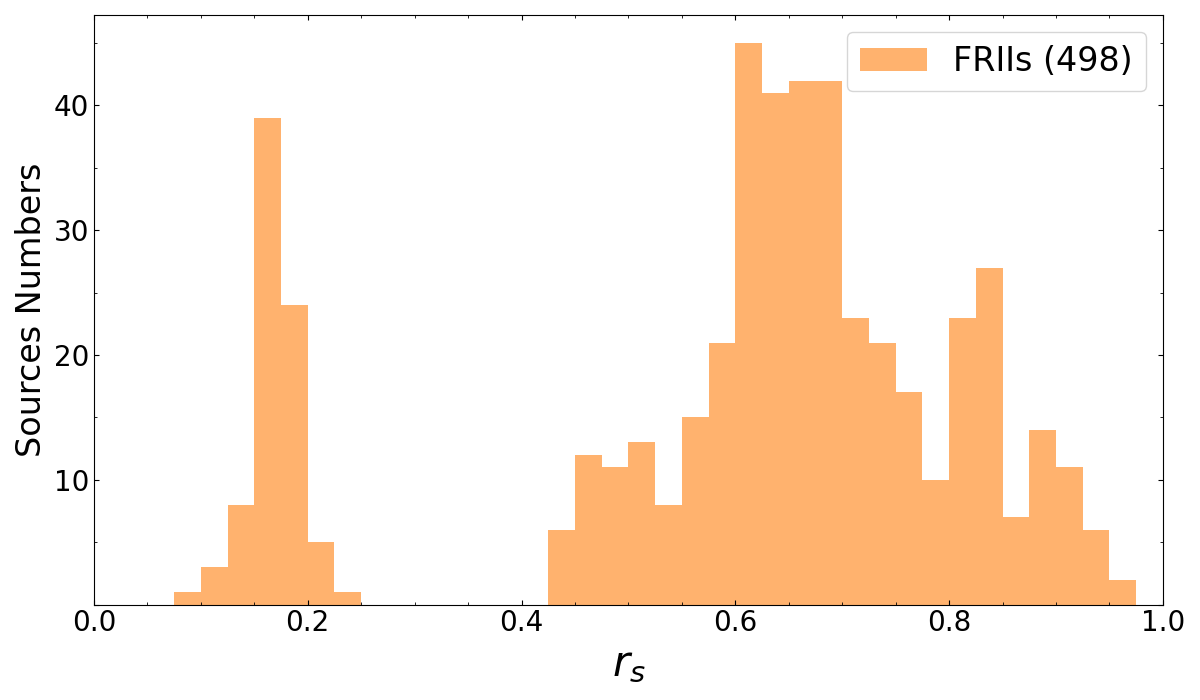
\includegraphics[width=0.9\linewidth]{Figure/Section 4/r_s_distribution0.png}
    \caption{
    Presents the distribution of $r_s$ for brightness threshold of 95\% (orange).
    }
    \label{fig:Figure12}
\end{figure}


As mentioned in previous section, we fit the morphologies of the RGs with ellipses, which can be described with the aspect ratio and the length of major axis.
The distribution of the aspect ratios for our FRI and FRII sources are shown in \autoref{fig:Figure7}. 
Generally, for both FRI and FRII, the source number peaks at about 0.3 and decrease to almost zero at extreme cases with the ratios about 0.1 or 0.9.
Compared to FRII sources which exhibit a distinct peak in aspect ratio, the distribution of FRI sources resembles more of a plateau, increasing and decreasing abruptly at 0.1 and 0.6, and decreases only gradually in the region where the ratio exceeds 0.6.

The length of major axis indicate the max scale of the source. For the sources with identified optical counterparts, their redshifts and distances are available, and therefore the intrinsic physical scales of the radio emission can be inferred.  The distribution of the physical scales are shown in \autoref{fig:Figure8}.
It can be seen that the sizes of FRIIs are much larger than those of FRIs on average, with the former peaking at about 200 kpc and the latter about 50 kpc.
It is seldom for FRIs to extend to 300 kpc and mostly less than 120 kpc, while for FRII size about 300 kpc is not special.

%When locating the principal component direction in \autoref{sec:Section3_1}, this direction can be used to trace the maximum separation distance between the two extremities of the RG system. 
%Given that the optical counterpart has already been localized, its redshift can be determined; this enables the approximate estimation of the RG system’s intrinsic physical scale through corrections based on cosmological models. \autoref{fig:Figure8} shows the distribution of these intrinsic physical scales. The distributions immediately reveal that the physical scales of FRIIs generally exceed those of FRIs: as shown in the subplots, FRIs peak near 50 kpc, while FRIIs exhibit a peak around 200 kpc.
Here, we fitted the distribution of the scales, \textbf{and normalized them into unit so that the probability for sources of certain sizes can be estimated}, which are expressed as:
\begin{equation} 
\makebox[\linewidth]{$\mathrm{Y}(X) = A\frac{1}{X \sigma \sqrt{2\pi}} \exp\left(-\frac{(\ln X- \mu )^2}{2\sigma^2}\right).$}
\end{equation}
For the FRIs the fitting yields,
$A \approx 3.817 \times 10^3,\  \sigma \approx 0.635,\ \mu \approx 4.392 \ $;
for the FRIIs the fit yields 
$ A \approx 2.899 \times 10^4,\  \sigma \approx 0.699,\ \mu \approx 5.501 \ $.



\begin{figure*}[!htbp]
    \centering
    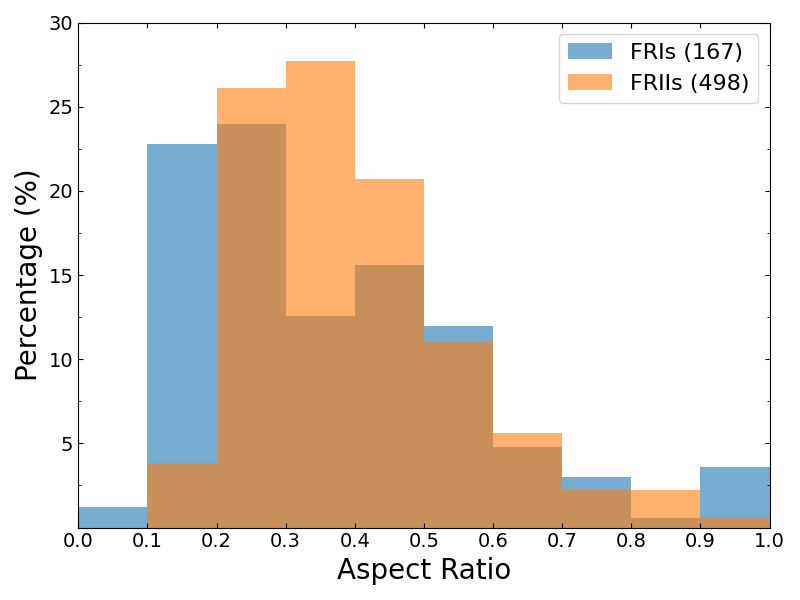
\includegraphics[width=0.9\linewidth]{Figure/Section 4/AxisRatio.png}
    \caption{The vertical axis represents the number of RGs, and the horizontal axis represents the axial ratio of the fitted ellipses. Left Panel: Matching FRIs; Right Panel: Matching FRIIs.}
    \label{fig:Figure7}
\end{figure*}
\begin{figure*}[!htbp]
    \centering
    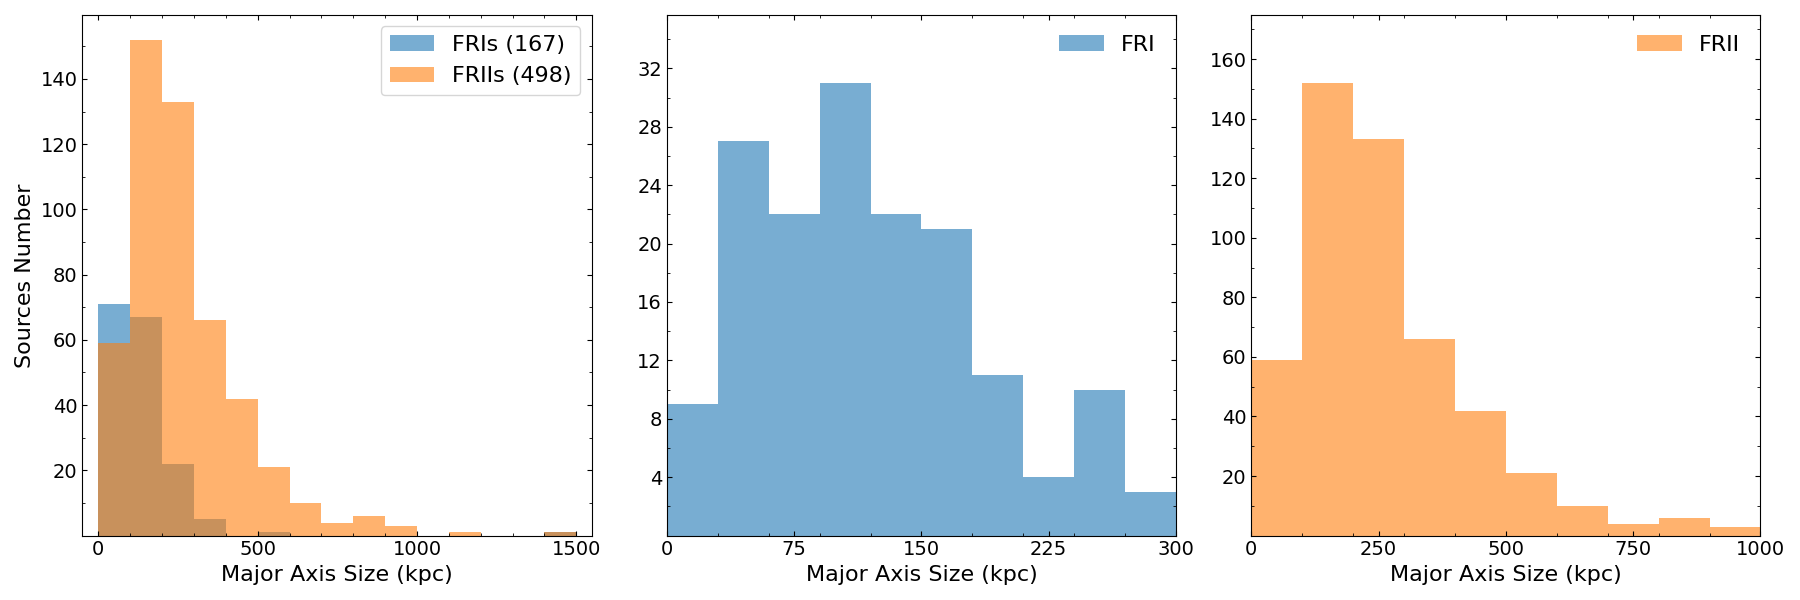
\includegraphics[width=0.9\linewidth]{Figure/Section 4/Max_Scale_Distribution.png}
    \caption{The distribution of physical scales of RGs classified by FR type. The blue and red histograms show the corrected maximum scales for FRIs and FRIIs, respectively. }
    \label{fig:Figure8}
\end{figure*}


% Nodes分布特征
\subsection{The Node Numbers }\label{sec:Section4_2}

%\cite{mizuno_recollimation_2015} investigated the mechanism and numerical simulations of jet recollimation: when AGN jets interact with their cosmic environment, they narrow and brighten over a characteristic length scale. During processing in \autoref{sec:Section3_3}, interest in knot structures emerged, leading to the incidental development of a counting method. This method is straightforward: building on the aforementioned flood-filling approach, a threshold (as a percentage of the central clump's maximum brightness) is incrementally increased to constrain the RG extent. Distinct knots are revealed in this process\textemdash with rising thresholds, knots originally blended in lobes gradually separate, then fade, leaving only the bright core (similar to \autoref{fig:Figure9}). A key distinction must be clarified before presenting results: "knot" refers to clumpy structures excluding the bright core in FRI sources, whereas "node" includes the bright core.

Increasing the threshold for the flood-filling approach incrementally, some isolated radio structures can be found in FRIs, as shown in \autoref{fig:Figure9}.
These structures are larger than one pixel and remain exist when the increment of the threshold is higher than 2 percent, which are not likely to be due to fluctuation, and should be the radio knots. If the threshold is very small, the whole radio structure constitute one or two large nodes, showing the morphology of the radio sources. 
If the threshold is about 1, the number of nodes may become zero as there is only one pixel, which is of highest luminosity.


The total knots in FRIs and FRIIs are investigated as shown in \autoref {fig:Figure10}. 
For FRI sources, when the threshold increases to 10\%, more and more sources start to show knots of the lowest power
Three curves with distinct colors depict the number of RGs with different architectures as a function of the brightness threshold.
The variation in the number of nodes with the threshold is represented by a solid line; the dash-dot line, which exhibits a negative correlation with solid line, denotes the variation in the number of RGs characterized by a single node (i.e., pure nuclear clumps); and the number of RGs identifiable by the algorithm is indicated by the middle dotted line. Herein, the statistical sample comprises 270 FRIs. 
Due to the constraints of the flood-filling algorithm implemented in this study, a contour-enclosed area that is excessively small is not recognized as a distinct region. Consequently, prior to the 75\% brightness threshold, a small number of FRIs with near-compact structures induce a slight decline in the dotted line. Beyond 75\%, further increases in the brightness threshold result in an increasing number of FRIs retaining only an extremely small bright central region, leading to an accelerated downward trend of the dotted line. Meanwhile, the solid line in the right panel exhibits two primary trends: an accelerated growth in the number of sub-clumps before 10\%, followed by a fluctuating decrease between 10\% and 70\%. In contrast, the dash-dot line illustrates that the number of FRIs without substructures drops rapidly before 10\% and fluctuates between 10\% and 70\%. Eventually, driven by the downward trend of the dotted line, both the solid and dash-dot line experience a combined accelerated decline, and all FRIs eventually evolve into pure nuclear clumps.

% 讨论Node的变化是否合理——排除涨落的特征
However, could the variation in the number of nodes potentially be attributed to occasional brightness fluctuations? By nature, random fluctuations are characterized as unpredictable small-amplitude variations, corresponding to a significantly low Coefficient of Variation (CV). In contrast, structural changes manifest as systematic variations with inherent regularity, where the CV assumes a moderate value and is accompanied by distinct trend-like features. 
Thus, the CV can be employed as a quantitative metric to discriminate between fluctuations-driven and structure-driven variations. For non-negative random variables following a normal distribution, the CV is defined as the ratio of the sample standard deviation to the sample mean, i.e., $CV =\sqrt{\mathrm{Var}}/\mathbb{E} \ ,$ where $\mathrm{Var}$ denotes the sample variance and $\mathrm{E}$ represents the sample mean. 
A total of 124 FRIs have a brightness variation coefficient of $CV=0$, and all these RGs consistently exhibit a node number distribution of 1; after excluding these sources, among the remaining 146 samples, 133 RGs ($\approx 91.1\%$) show persistent knots over continuous brightness intervals of more than 2\%, while 142 RGs ($\approx 97.3\%$) in these samples have their CV falling within the range of $0.1 \sim 0.8$.


\begin{figure*}[!htbp]
    \centering
    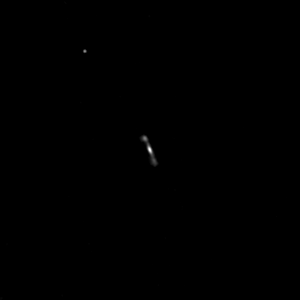
\includegraphics[clip, trim=125 125 125 125, scale=1, width=0.25\linewidth]{Figure/Section 4/Knot_ori.png}
    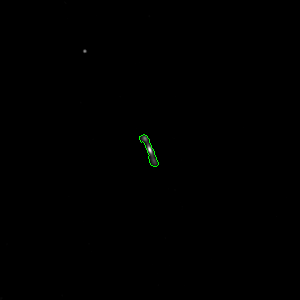
\includegraphics[clip, trim=94 94 94 94, scale=1, width=0.25\linewidth]{Figure/Section 4/Knot_0.5.png}
    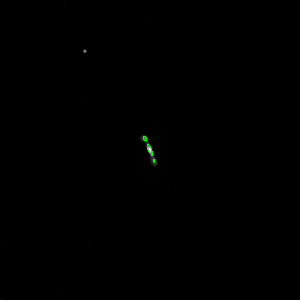
\includegraphics[clip, trim=94 94 94 94, scale=1, width=0.25\linewidth]{Figure/Section 4/Knot_25.png}
    \caption{A FRI type RG located at equatorial coordinates (R.A. 197.092°, Dec. 23.521°). As the threshold increases, four knots are exposed. Left: The original RG radio image (R.A. 178.47°, Dec. 38.197°);  Middle: The identified contour of RG, \textbf{threshold of 5\%????}, is shown with green line;  Right: The contours of knots are shown when the threshold is 25\%.}
    \label{fig:Figure9}
\end{figure*}

\begin{figure}[!htbp]
    \centering
    \begin{tabular}{cc}
        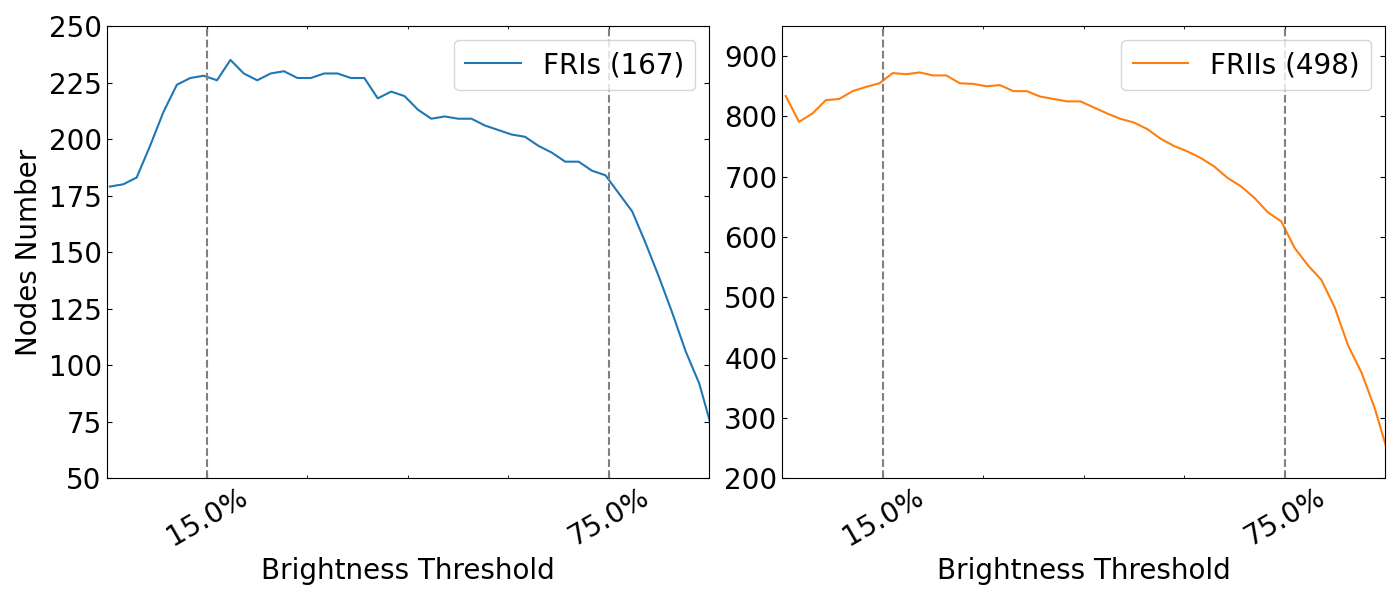
\includegraphics[width=0.9\linewidth]{Figure/Section 4/Node_Evolution.png}
        \end{tabular}
    \caption{Variation of counts of different types with brightness threshold. The horizontal axis represents the brightness threshold expressed as a percentage of the brightest point in RGs, and the vertical axis denotes the number of RGs or nodes.}\label{fig:Figure10}
\end{figure}
% \clearpage




\subsection{Brightness Stacking along the Central Lines of FRIIs}\label{sec:Section4_4}

In addition to the overall radio morphology, the intensity distribution provides more detailed information about the RGs. 
Here we use a curve referred as central line to describe the direction of the jet flow, and adopt the intensity along the line as the representative of the intensity distribution.
However, for FRIs, the radio emission distribute over a wide range, and the central line is not effective.
So we only investigated the central line in FRII sources.
\textbf{The left panel of \autoref{fig:Figure5} shows two examples of the identified central lines for the radio sources (RA... or source names) for cases of low and high aspect ratios???}. It can be seen that the central lines are feasible to mark the trajectories of the radio structure centers.

%\cite{turner_energetics_2015} previously proposed an evolutionary model for FRI/FRII radio AGNs and their mutual transitions. To reveal the dynamical mechanisms of jet-ambient medium interactions, they developed a comprehensive model that encompasses the supersonic, transonic, and subsonic phases of jet-cocoon expansion, alongside a comparative pure FRII model (where jets maintain supersonic expansion throughout their entire lifecycle). Thus, how can these characteristics be captured?
%In \autoref{sec:Section3_5}, we propose using the centerline to characterize the brightness distribution of RG. However, constrained by observational resolution, only the most  prominent regions can be focused on; nevertheless, stacking these prominent regions may reveal characteristics of the population evolution of FRIIs. 
%To investigate the brightness properties of cores and lobes, the centerline brightness distribution curves of all FRIIs (e.g., \autoref{fig:Figure5}) were acquired. 

We further explored the radio emission along the central line. To get a general picture of  

To calculate the 1.4 GHz radio luminosity, we use the formula cited in \cite{koziel-wierzbowska_identifying_2021} ($\alpha$ is adopted as 0.75, serving as the mean spectral index for sources detected at 1.4 GHz) 
 

To assess the error budget, three factors are considered in this work. First, the FIRST official website specifies a typical rms of 0.15 mJy, while rms values derived from cropped images deviate from this reference. Second, VizieR notes that for bright sources, the accuracy of Fpeak is limited to approximately 5\% due to systematic effects. Third, a code modification for pixel position bias correction is introduced, which simulates pixel position deviations in the calculation of the horizontal axis physical scale to estimate errors caused by pixel discretization. However, minor deviations from redshift and cosmological models are not considered. Additionally, the error propagation formula is applied to each calculation step. Finally, red shaded regions are used to represent the errors in \autoref{fig:Figure13}.
% 最终换算出来的单个RG最大光度范围大概是 1e28-1e32 W/Hz 居多，是否存在问题？
% 已解决，单个FRII类型的RG的光度范围实际上是1e26 - 1e29 W/Hz范围
% 光度范围过大，可以归结为“选取的中心线往往是RG最亮的位置”，所以换算得到的光度就比一般的RG更亮得多
Notably, as shown in \autoref{fig:Figure13}, the stacking curve ranges from $ 10^{31}\ W\ \text{Hz}^{-1}\ \text{kpc}^{-2} $ to $ 10^{33}\ W\ \text{Hz}^{-1}\ \text{kpc}^{-2} $. Given that the order of magnitude of the number of stacked RGs is approximately $ 10^{3} $, and the selected regions correspond to the brightest "central line" regions across the entire RGs, the derived luminosity exceeds the typical luminosity range of FRII galaxies, which is between $ 10^{25}\ W\ \text{Hz}^{-1}  $ to $ 10^{29}\ W\ \text{Hz}^{-1} $\citep[e.g.,][]{an_dynamic_2012}.



In the present work, we seek to verify Turner’s conclusions. Specifically, we split the center lines of FRIIs at their optical counterparts\textemdash thereby doubling the sample size\textemdash and then stacked the brightness distributions of all sample central lines, from which we derived the brightness stacking curve presented in \autoref{fig:Figure13}. The statistically derived brightness-stacked profiles of FRIIs exhibit structural similarity to their luminosity-size profiles: within 100 kpc of the optical counterpart, the brightness increases with distance until reaching a peak, followed by a steep decline where brightness decreases rapidly with increasing distance. Notably, the FRIs' population did not exhibit significant characteristics and thus are not presented herein.



% \begin{figure*}
%     \centering
%     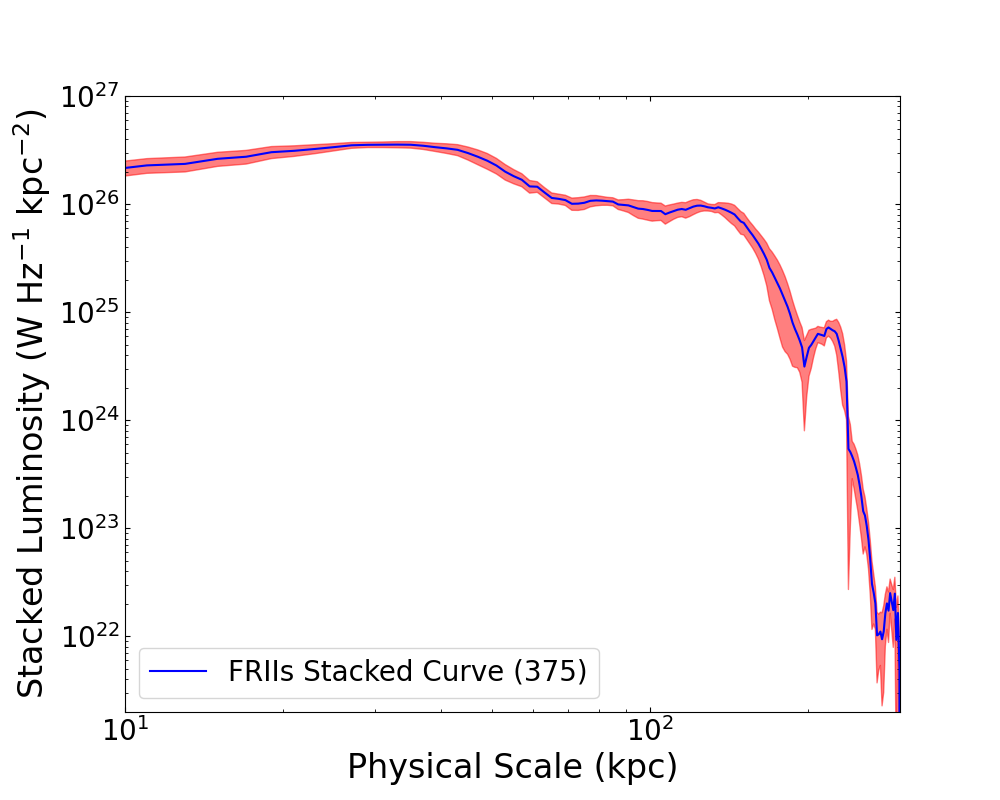
\includegraphics[width=0.45\linewidth]{Figure/Section 4/FR2_StackingCurve1.png}
%     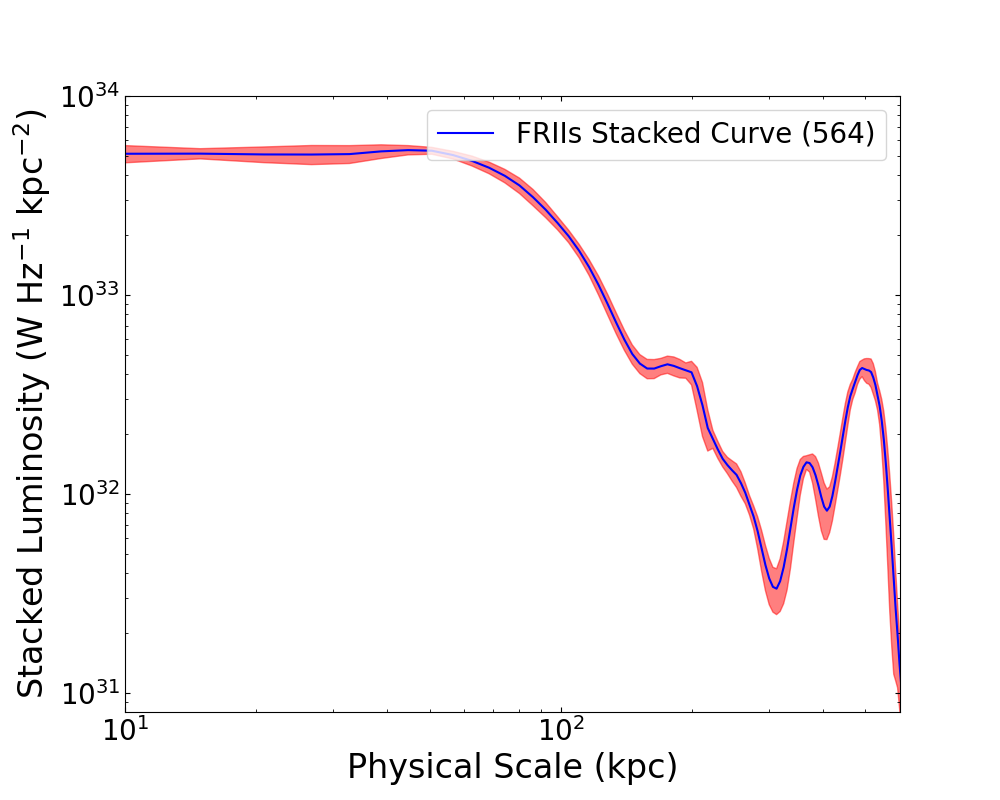
\includegraphics[width=0.45\linewidth]{Figure/Section 4/FR2_StackingCurve2.png}
%     \caption{The center line brightness stacking curve of FRIIs. The horizontal axis represents the distance from the extracted physical scales to the location of the optical counterparts of RGs; the vertical axis denotes the logarithmic luminosity.}
%     \label{fig:Figure13}
% \end{figure*}
\begin{figure}
    \centering
    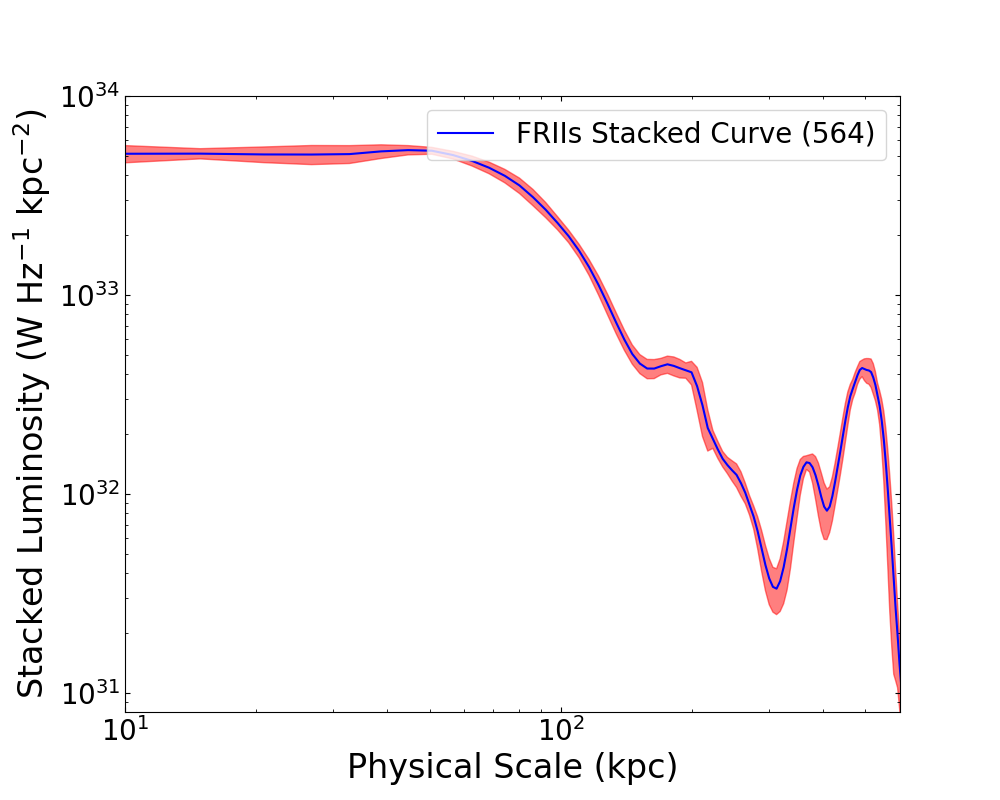
\includegraphics[width=0.9\linewidth]{Figure/Section 4/FR2_StackingCurve2.png}
    \caption{The center line brightness stacking curve of FRIIs. The horizontal axis represents the distance from the extracted physical scales to the location of the optical counterparts of RGs; the vertical axis denotes the logarithmic luminosity.}
    \label{fig:Figure13}
\end{figure}


% 伸长参数
\subsection{The Distribution of Elongation Parameter}\label{sec:Section4_5}

In \autoref{sec:Section4_3}, the method outlined for deriving the S value differs for FRIs, which implies that the $r_s$ values obtained for FRIs cannot be directly compared with those of FRIIs. Thus, the distribution of $r_s$ values for FRIs is not presented; an alternative parameter is employed in this section to compare FRIs and FRIIs.

Similarly, after the PCA direction is determined (see \autoref{sec:Section3_4}), the two points marking the RG’s maximum extent along this direction are identified as the maximum elongation value. The maximum distance perpendicular to the PCA direction, when divided by this maximum elongation value, yields the elongation parameter. Probability density distributions of the elongation parameter K are presented in the left panel of \autoref{fig:Figure14}, while the half-opening angle ($\theta$) estimated via $\arctan(1/K)$ and its corresponding probability density distribution are displayed in the right panel. The probability densities of K for FRIs and FRIIs appear relatively similar; however, those of $\theta$ for the two classes exhibit distinct differences.

% Both FRI and FRII show multiple peaks in their K distributions, with shared peaks at ~K=2.2, 3.2, and 4.2. FRI, however, has an additional prominent peak at \(K \approx 1.6\) (absent in FRII), suggesting a potential FRI subpopulation with smaller K values. If these correspond to older jet remnants, their jets\textemdash whether propagating through poloidal or helical magnetic fields \citep{barniol_duran_simulations_2017}\textemdash may become randomized by subsequent AGN activity or prolonged environmental interactions, reducing the directional coherence and elongation signatures typical of younger jets. This substructure may align with Andreasyan’s conjecture: they noted that "the maximum of the distribution of the FRII RGs lies at \(K \approx 2.8\) and the peak for the FRI sources is at \(K \approx 2.2\)", and we obtain similar peaks. However, our derived K distribution functions differ appreciably in structure with their result, implying that beyond specific characteristic peaks, the actual elongation parameter distribution curves of FR sources vary significantly with sample selection criteria.


\begin{figure*}
    \centering
    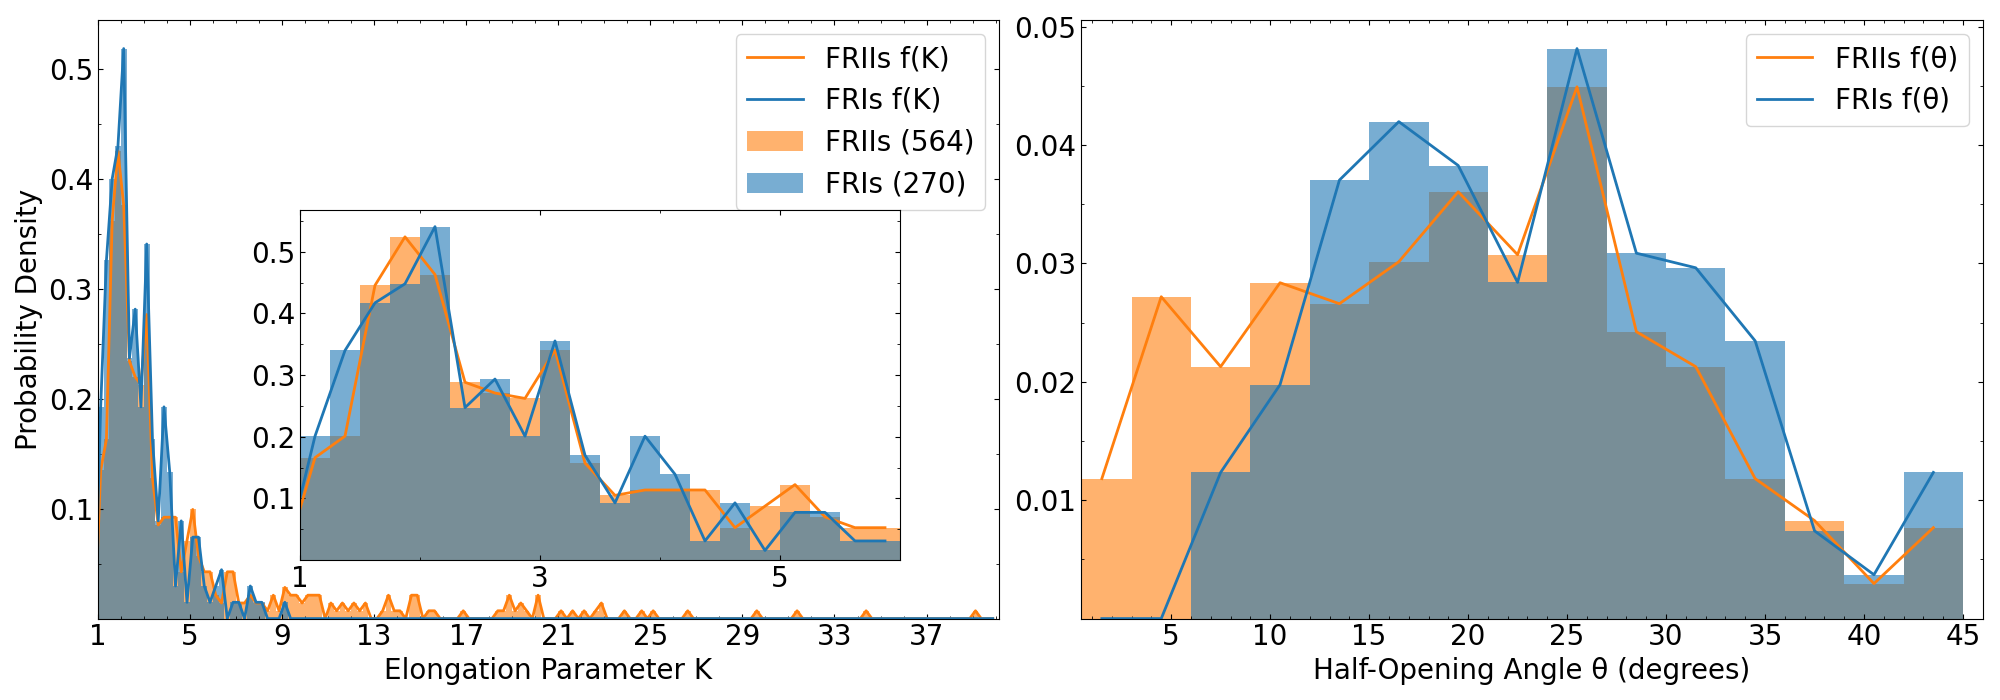
\includegraphics[width=0.9\linewidth]{Figure/Section 4/ProbabilityDensity.png}
    \caption{Left Panel: Probability density distribution of the elongation parameter K; The horizontal axis represents K, and the vertical axis denotes the probability density of K; Histogram bins for K are set at intervals of 0.25, with the corresponding curve $f(K)$ representing the probability density function of K; Red and blue colors correspond to FRIs and FRIIs, respectively. Right Panel: Probability density distribution of the half-opening angles ($\theta$) of RGs estimated using K; The horizontal axis represents the $\theta$, and the vertical axis denotes the probability density of the $\theta$; Histogram bins for the $\theta$ are set at intervals of $3^\circ$ , with the corresponding curve $f(\theta)$ representing the probability density function of the $\theta$.}
    \label{fig:Figure14}
\end{figure*}


\section{Discussion}\label{sec:Discussion}

\subsection{The Deviations in Procedure}\label{sec:Section5_1}
% 大概介绍一下对源处理的偏差
% 1.光学对应体匹配
In practice, genuine optical counterparts may remain unmatched due to observational limitations. Consequently, a substantial fraction of RGs lacking matched optical counterparts must be excluded from our program. The matching status of optical counterparts is illustrated in \autoref{fig:Figure15}.
% ——要绘制图片展示匹配的光学对应体数目：1，多，0。然后讨论一下和Data中FIRST匹配数据的偏差。
\begin{figure}
    \centering
    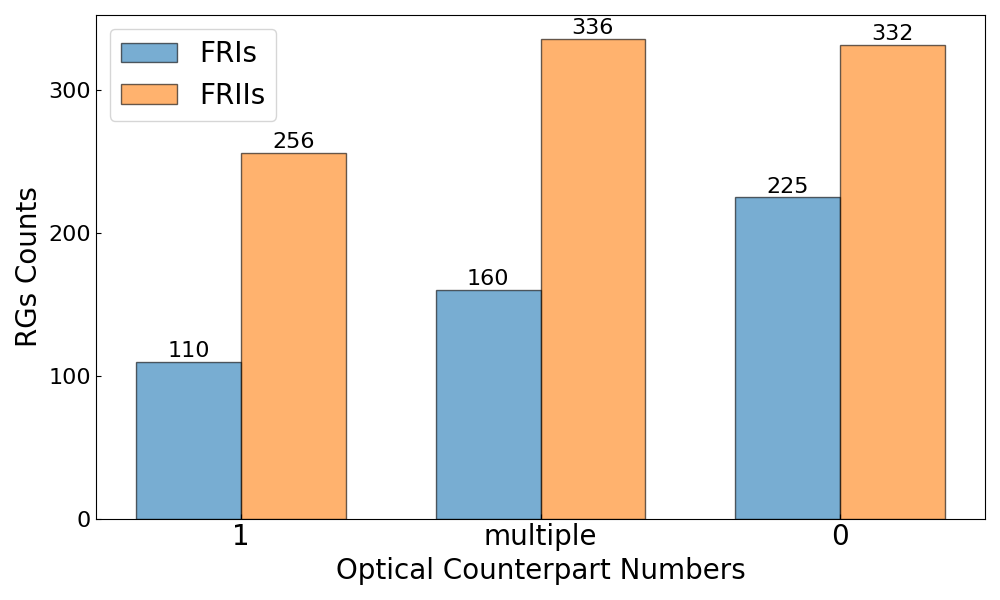
\includegraphics[width=0.9\linewidth]{Figure/Section 5/OpticalCounterpartCountDistributions.png}
    \caption{This figure illustrates the distribution of RGs during the search for their optical counterparts. The two colored labels correspond to FRI/FRII type RGs, respectively. The horizontal axis represents the number of optical counterparts detected for each RG: optical counterparts with a detection count of 1 are relatively more reliable than those with a count of "multiple", and RGs with an optical counterpart count of 0 will be excluded from our subsequent analysis. The vertical axis denotes the number of RGs.}
    \label{fig:Figure15}
\end{figure}


% 2.argue一下星系倾角问题！从各向同性出发，参考其他人的文章。
In observational studies of radio galaxies, the inclination angle problem has long been a core challenge plaguing astronomers. The inclination angle is defined as the angle between the axis of symmetry of a radio galaxy and the observer’s line of sight, and this seemingly straightforward geometric parameter actually encapsulates highly complex physical information. Since the observed radio galaxy images are essentially the projection of three-dimensional structures onto the two-dimensional celestial sphere, different inclination angles can result in entirely distinct observed morphologies for the same intrinsic structure \citep{reynolds_projection_1980}. The degeneracy arising from this projection effect renders the extraction of true physical parameters from observational data extremely challenging. With the continuous advancement of technology, several methods based on isotropy to infer the inclination angle have emerged \citep[e.g.,][]{schmitt_jet_2001,drouart_jet_2012,oei_discovery_2022}, but these approaches impose non-trivial requirements on observational data and telescope resolution\textemdash requirements that are not easily satisfied in the work presented in this paper.

% 3.高斯椭圆的结构其实也有问题
Additionally, Gaussian elliptical fitting for component extraction requires attention. With fewer constraints, its fitting accuracy may decrease, necessitating extensive manual inspection to identify poor fits and ensure high-quality source extraction. Thus, complex Gaussian fitting is unsuitable for large-scale survey data analysis; it may even cause catastrophic errors when applied to highly distinct RGs. However, it remains adequate for component extraction in simple scenarios. Notably, when constraining component division for RGs, we adopted a strict 95\% brightness threshold for FRIIs but only 80\% for FRIs. This is due to the general characteristics of FR types: FRIs often have faint, diffuse edge structures that severely hinder key region identification, whereas the more regular structure of FRIIs allows for stricter constraints. There may be cases of failure to match an ellipse. The difference in the number of FRIIs in \autoref{fig:Figure12} is precisely because some RGs cannot achieve 95\% coverage by an ellipse due to their diffuse structures. However, this issue is alleviated when the coverage threshold is reduced.


% 4.中心线定位并不准确
In this study, the BSF is utilized to locate the center line; however, this method may introduce deviations. Specifically, this localization process is analogous to pruning, which tends to eliminate "extraneous branches" in regions with complex structures. Naturally, the structural features exhibited in complex regions undergo a more pronounced simplification than those in simple regions. Our method demonstrates advantages over ridge line-based approaches: specifically, the quality of ridge lines is highly dependent on image preprocessing steps, and they are less suitable for RG systems featuring large gaps or curved head-tail structures \citep[e.g.,][]{barkus_application_2021,clews_radio-loud_2025}.



% 介绍堆叠曲线在一定区域内不可靠的情况
% Additionally, given that FRII sources typically have dim or absent core regions relative to their lobes, combined with the scarcity of large-scale data, the brightness-stacked profiles near core regions and in outer large-scale lobes are unreliable. For instance, the profiles of FRIIs exhibit obvious abrupt linear transitions around 1 kpc in their central regions\textemdash a phenomenon attributed to the fact that the brightness\textemdash distance grid near these transition sites is smaller than the pixel resolution of FIRST.


In our previous work, we have conducted research on the distribution characteristics of RGs. It can be noted that both the redshift distribution in \autoref{fig:Figure3} and mass distribution in \autoref{fig:Figure4}, the RGs exhibit concentrated clustering characteristics, with individual sources showing significant deviation from the primary cluster; however, ignoring extreme objects and considering the overall pattern, the distribution range of FRIIs is distinctly broader than that of FRIs. In terms of redshift distribution, FRIs are largely confined to regions below $z \sim 0.5$, while FRIIs extend smoothly from $z \sim 0$ to approximately $z \sim 1.5$. This likely indicates that FRIs, being intrinsically dimmer than FRIIs, are detectable only at relatively low redshifts. Regarding mass distribution, the ranges of central black hole mass and stellar mass for FRIIs are wider than those for FRIs, yet their distribution peaks are notably similar: Central black hole masses cluster near $10^{8.5} M_\odot$, and stellar masses cluster near $10^{11.5} M_\odot$. These deviations may arise from the sensitivity characteristics of telescope observations or could indeed reflect inherent differences in the physical properties of these RGs.



\subsection{Similar Mechanism of Morphological Evolution?}\label{sec:Section5_2}
% 提及应用前景
The original objective of this project is to extract statistical parameters that can characterize the structure of RGs from the sample distributed at 1.4 GHz. The Murchison Widefield Array has presented deep-exposure images of EoR in specific sky fields \citep{offringa_parametrizing_2016}, and has also demonstrated the existence of dense extragalactic sources. Such extragalactic sources serve not only as the observational background for the 21 cm forest but also may act as foreground contaminants. Once a basic understanding of such extragalactic foreground contamination is established, consideration can be given to methods for its subtraction. Some methods of foreground source modeling need subtract bright sources at the first \citep{di_matteo_radio_2002,di_matteo_21-cm_2004}.  A qualitative understanding of the structure of foreground sources is required; for example, Independent Component Analysis of \cite{chapman_foreground_2012} relies on observational constraints and physical models derived from RGs. 


% 椭圆轴比聚集于0.25，FRIs比FRIIs更弥散
To characterize the structures of RGs, we employed elliptical fitting for parameter extraction. In \autoref{sec:Section3_6}, elliptical structures can be fitted to FR-type RGs, with the axial ratios of these ellipses subsequently computed. \autoref{fig:Figure7} presents binned histograms of axial ratios for FRIs and FRIIs, constructed with the same number of bins. Although the sample size of FRIs is smaller than that of FRIIs, the overall axial ratio distribution of FRIs is considerably more dispersed. Given that FRIIs typically host more powerful central engines than FRIs, their jets may be less susceptible to environmental effects. Here, a distinct clustering in the FRII distribution is evident, suggesting that FRII radio lobe structures naturally tend toward axial ratios approaching 0.25. Notably, the peak of the FRI distribution also lies near an axial ratio of 0.25. In \autoref{fig:Figure8}, the discrepancy in physical scale distributions between FRIs and FRIIs is clearly observable and remarkably large; nevertheless, both the axial ratio and elongation parameter exhibit similar distribution patterns across the two classes. This observation implies the existence of a shared mechanism of morphological evolution in FR-type RGs.




\subsection{The Phenomenon of Brightness Stacking Curve}\label{sec:Section5_3}

% 事实上凸起不够显著，来自望远镜的偏差
First, we introduce FRIIs. The brightness stacking curve of FRIIs show brightness distribution in our study is not enough significantly compared with the pronounced protuberance observed in Turner's work. Apart from biases arising from the matching of optical counterparts and RGs, an intuitive explanation lies in observational sensitivity: the extended structures of radio AGNs may be underestimated due to insufficient sensitivity, \cite{shabala_delayed_2017} simulated model parameters for three VLBI-detected AGNs (MJV 02278, MJV 16230, and MJV 16427) and compared brightness-versus-physical-scale curves under varying telescope sensitivities to illustrate this effect.

Then we can see that the inaccuracy in centerline positioning is reflected in the stacked curves: if all identified optical counterparts of RGs could be precisely aligned with the centers of radio structures, the physical scale distribution of FRIIs in \autoref{fig:Figure13} should in principle be half of that in \autoref{fig:Figure8}. This indicates a significant deviation between the centerlines derived in this work and the optical counterparts. Potential explanations include misidentified optical counterparts for some RGs (even though we prioritized those proximate to radio structure centers as much as possible) and biases arising from the inclination angles of RGs and the Doppler effect. However, regions of substantial radio brightness adjacent to the optical counterparts are relatively reliable: Consistent with general understanding, while the radio lobes of FRIIs are brighter, their spatial distribution is random; by contrast, the faint central sources of FRIIs, when stacked together, should indeed be brighter than the lobe areas. Other prominent features can be interpreted as radio-active regions. In contrast to the distinct characteristics of FRIIs, the unilateral brightness stacking profiles of FRIs lack analogous prominent features, thus other statistical approaches for FRIs should be considered.


% 讨论一下Knots分布的故事
\subsection{The Steady Change of Knots}\label{sec:Section5_4}

Notably, for knot structures in FRIIs\textemdash such as Hot Spots describable via shock processes, and multiple Hot Spot configurations  (e.g., Double-Double radio galaxies) explainable as relics of past AGN activity\textemdash most FRIs exhibit significantly lower luminosity than FRIIs. The central engine power of FRIs is often insufficient to sustain jets at FRII-scale lengths, rendering Hot Spot models inapplicable to FRIs. Accordingly, knots are treated here as a descriptive feature for FRIs, and we shift our perspective from linear to surface-based characterizations.


Evidently, during observations, we have observed two distinct types of knots\textemdash the bright core of FRIs and the hotspots of FRIIs. However, dedicating specific discussion solely to FRII knots may not hold significant value at this point, as both double hotspots and double-double lobe configurations have already emerged as independent classification frameworks: the prevailing view regarding double-double lobes posits the potential occurrence of multiple jet outbursts, which re-energize remnants from previous outbursts, thereby forming two pairs of hotspots; additionally, the presence of more complex hotspot structures may similarly stem from multiple outbursts or limitations imposed by telescope sensitivity. In contrast to FRIIs, FRIs are fundamentally considered core-dominated in radiative luminosity, while FRII structures span a broad range from low to high brightness, whereas FRIs generally appear only in low-brightness intervals. This implies that either environmental influences prevent the establishment of bright extended structures in RGs, or the AGN power is insufficient to support extended jets interacting with the cosmic environment. Based on this a priori hypothesis, we are filled with curiosity regarding the knots observed in FRIs.


% 对nodes分布的详细介绍
In the right panel of \autoref{fig:Figure10}, the trends of the three curves (solid line, dotted line, dotted line) as the brightness threshold increases reveal the characteristics of the radio brightness structures of RGs:
\begin{itemize}[label=•]
    
    \item For the solid line (tracking node count), between ~10\% and 75\% of the peak brightness, the node count decreases relatively uniformly (the coefficient of determination for the best-fit line is ~0.96, likely due to the predominant distribution of knot brightness within this range), with minor fluctuations in the total number of nodes/knots and node-bearing RGs.
    
    \item The dotted line (recording the number of RGs with recognized nodes) shows a slight decline at thresholds below 0.5\% and above 75\%—attributable to incomplete filtering of FRI systems (characterized by uniformly low luminosity and ambiguous brightness) in previous analyses—indicating that knot variation is unaffected by RG quantity. It decreases rapidly beyond 75\% because algorithmic limitations hinder the recognition of points with excessively narrow brightness ranges as nodes.
    
    \item The dash-dot line (illustrating sources with pure nuclear clump) exhibits fluctuations stemming from the "disintegration effects" of FRI core clumps—where multiple regions of non-uniform brightness gradually emerge within initially large clumps during flood-filling—and this process, alongside the discontinuous lobes around FRIs, represents the sole contributor to the node count.

\end{itemize}


% 介绍recolllimation—— knots数量真的跟recollimation无关吗？
How do AGN jets interact with their cosmic environment? A variety of physical processes regulate the dynamics and stability of these jets. As the initially overpressured jet streams away from the galactic center, its pressure decreases with increasing distance from the jet base. Eventually, it reaches a critical point where the jet pressure drops below the external environmental pressure. This pressure mismatch can cause the jet to undergo brightening—a phenomenon termed recollimation \citep[e.g.,][]{mizuno_recollimation_2015}. Furthermore, knots observed in NGC 2663 offer evidence for recollimation in FRI RGs \citep{velovic_collimation_2022}. However, in our dataset, it is clear that not all sources exhibit the trait that "more knots imply better collimation of FRI lobes." Manual inspection of our data further confirms that no correlation exists between a greater number of nodes and improved collimation of RG structures.




\section{Conclusions and Future} \label{sec:Conclusions and Future}

\subsection{Conclusions}\label{sec:Conclusions}

The objective of this work is to integrate existing research methodologies to conduct a deeper geometric analysis of RG structures based on FR-classified 1.4 GHz images.

The prevailing perspective on jets and radio lobes predominantly attributes their physics to shock-initiated processes. Within this consensus, we propose that elliptical geometries can effectively characterize FR-classified RGs. To derive optimally constrained elliptical structures, we employed Flood-filling algorithms, optical counterpart matching, and center-line construction, ultimately generating tailored elliptical models for FRI and FRII morphologies. Crucially, our methodology aims to develop a universal framework adaptable to diverse RG shapes, not limited to ellipsoidal forms. Consequently, we identified four distinct descriptive perspectives for RGs in the discussion section.


Our analysis can be summarised as follows:

\begin{itemize}[label=$\star$]

    \item From our perspective, we performed a statistical analysis on the geometric morphology of RGs, including their ellipticity axis ratio, physical scale, elongation parameter, and estimated half-opening angle. Besides refreshing our understanding of FR types, this study further quantitatively reaffirms the differences between FR I and FR II.
    
    \item The second perspective concerns the enumeration of knots in FRIs. Compared to the hotspots triggered by the relatively more powerful central engines of FRIIs, FRIs, despite their dimmer nature, also exhibit knots to a certain extent, though the role of these knots appears less significant. However, during the statistical analysis of knots, we observed that the number of knots within specific brightness intervals achieves a remarkable equilibrium, decreasing overall at a steady rate.
    
    \item Subsequently, we employed the classical $r_s$ method to analyze the sample, noting that FRIIs exhibit a substructure in the region where $r_s$ < 0.4, which arises from the significant outflow effects occurring at the hot spot.
    
    \item Finally, brightness stacked profiles. By leveraging the requirement to locate optical counterparts, we derived a curve describing both geometric and brightness characteristics of RGs—namely, the center line. Subsequently, stacking the brightness distributions of center lines from a sufficient sample size naturally reveals the average radiatively active regions. FRIIs demonstrate that average luminosity initially increases with physical scale, peaks, then decreases monotonically\textemdash a characteristic aligning closely with \cite{turner_energetics_2015} predicted dynamical model for FRIIs.
    
\end{itemize}

Integrating these perspectives collectively, this work provides improved clarity on the structural properties and evolutionary mechanisms of FR-classified RGs.




\subsection{Future}\label{sec:Future}

Future research should prioritize developing additional theoretical frameworks to explore the significant commonalities between FR I and FR II type RGs, which will substantially deepen the understanding of large-scale jet structures. A key direction lies in identifying the most critical parameters to establish a more authoritative classification system for RGs. Moreover, existing quantitative analyses under the FR classification framework remain superficial, so future progress must rely on more robust theoretical models and high-sensitivity observations targeting large-scale radio structures as foundational support to gain clearer insights into their intrinsic nature.


This work is anticipated to undergo further development and support simulation efforts in future research, including modeling jet structures for different RGs to refine the authentic jet-lobe morphologies observed by various telescopes. Furthermore, radio lobe structures may exhibit relevant interactions with the interstellar medium or intracluster medium; the description of these structures can be used to characterize the interactions between jets and the medium, and also reflect the kinematic components of the intergalactic medium as well as the characteristics of host galaxies. Additionally, special types of RGs will also be key research directions in the future, such as Giant RGs and Hybrid Morphology RGs.

%Additionally, the fine sub-kiloparsec scale structures of radio-quiet AGNs \citep[e.g., those detected in J0802+4643][]{vardoulaki_fr-type_2021} can fill the statistical gaps in this work, and the development of future radio telescopes will further expand the understanding of RG structures.


% 另外，曾经考虑过将连续中心线参数化，变为一组可描述射电结构的参数，但由于中心线定位并不清晰，用参数化描述的结果并不好
% ——强烈的核活动也会影响星际介质和星际电介质的星形成历史及其特性，从而成为它们宿主及其大尺度环境演化的基本成分。

\bibliographystyle{aa.bst}
\bibliography{BibDir/Introduction.bib,BibDir/Data,BibDir/Method,BibDir/Discussion}
% \bibliography{BibDir/Data,BibDir/Method,BibDir/Discussion}
% \bibliography{BibDir/Introduction.bib}
\begin{appendix}
\section{Alternative thread identification}\label{app:Alt} 




\end{appendix}






\end{document}

